\documentclass[sigplan,10pt,review,anonymous]{acmart}\settopmatter{printfolios=true,printccs=false,printacmref=false}
  \usepackage{graphicx}
  \usepackage{listings}
  \usepackage{enumitem}
  \newcommand{\MC}{MakeCode\ }
  \newcommand{\MCN}{MakeCode}
  \setlist[itemize]{leftmargin=*}
  \lstset{ %
  language=C++,                % choose the language of the code
  basicstyle=\footnotesize,       % the size of the fonts that are used for the code
  numbers=left,                   % where to put the line-numbers
  numberstyle=\footnotesize,      % the size of the fonts that are used for the line-numbers
  stepnumber=1,                   % the step between two line-numbers. If it is 1 each line will be numbered
  numbersep=5pt,                  % how far the line-numbers are from the code
  backgroundcolor=\color{white},  % choose the background color. You must add \usepackage{color}
  showspaces=false,               % show spaces adding particular underscores
  showstringspaces=false,         % underline spaces within strings
  showtabs=false,                 % show tabs within strings adding particular underscores
  frame=single,           % adds a frame around the code
  tabsize=2,          % sets default tabsize to 2 spaces
  captionpos=b,           % sets the caption-position to bottom
  breaklines=true,        % sets automatic line breaking
  breakatwhitespace=false,    % sets if automatic breaks should only happen at whitespace
  escapeinside={\%*}{*)}          % if you want to add a comment within your code
  }
  
    %% For double-blind review submission, w/ CCS and ACM Reference
    %\documentclass[sigplan,10pt,review,anonymous]{acmart}\settopmatter{printfolios=true}
    %% For single-blind review submission, w/o CCS and ACM Reference (max submission space)
    %\documentclass[sigplan,10pt,review]{acmart}\settopmatter{printfolios=true,printccs=false,printacmref=false}
    %% For single-blind review submission, w/ CCS and ACM Reference
    %\documentclass[sigplan,10pt,review]{acmart}\settopmatter{printfolios=true}
    %% For final camera-ready submission, w/ required CCS and ACM Reference
    %\documentclass[sigplan,10pt]{acmart}\settopmatter{}
    
    
    %% Conference information
    %% Supplied to authors by publisher for camera-ready submission;
    %% use defaults for review submission.
    \acmConference[PL'17]{ACM SIGPLAN Conference on Programming Languages}{January 01--03, 2017}{New York, NY, USA}
    \acmYear{2017}
    \acmISBN{} % \acmISBN{978-x-xxxx-xxxx-x/YY/MM}
    \acmDOI{} % \acmDOI{10.1145/nnnnnnn.nnnnnnn}
    \startPage{1}
    
    %% Copyright information
    %% Supplied to authors (based on authors' rights management selection;
    %% see authors.acm.org) by publisher for camera-ready submission;
    %% use 'none' for review submission.
    \setcopyright{none}
    %\setcopyright{acmcopyright}
    %\setcopyright{acmlicensed}
    %\setcopyright{rightsretained}
    %\copyrightyear{2017}           %% If different from \acmYear
    
    %% Bibliography style
    \bibliographystyle{ACM-Reference-Format}
    %% Citation style
    %\citestyle{acmauthoryear}  %% For author/year citations
    %\citestyle{acmnumeric}     %% For numeric citations
    %\setcitestyle{nosort}      %% With 'acmnumeric', to disable automatic
                                %% sorting of references within a single citation;
                                %% e.g., \cite{Smith99,Carpenter05,Baker12}
                                %% rendered as [14,5,2] rather than [2,5,14].
    %\setcitesyle{nocompress}   %% With 'acmnumeric', to disable automatic
                                %% compression of sequential references within a
                                %% single citation;
                                %% e.g., \cite{Baker12,Baker14,Baker16}
                                %% rendered as [2,3,4] rather than [2-4].
    
    
    %%%%%%%%%%%%%%%%%%%%%%%%%%%%%%%%%%%%%%%%%%%%%%%%%%%%%%%%%%%%%%%%%%%%%%
    %% Note: Authors migrating a paper from traditional SIGPLAN
    %% proceedings format to PACMPL format must update the
    %% '\documentclass' and topmatter commands above; see
    %% 'acmart-pacmpl-template.tex'.
    %%%%%%%%%%%%%%%%%%%%%%%%%%%%%%%%%%%%%%%%%%%%%%%%%%%%%%%%%%%%%%%%%%%%%%
    
    
    %% Some recommended packages.
    \usepackage{booktabs}   %% For formal tables:
                            %% http://ctan.org/pkg/booktabs
    \usepackage{subcaption} %% For complex figures with subfigures/subcaptions
                            %% http://ctan.org/pkg/subcaption
    
    \usepackage{courier}

    \begin{document}
    
    %% Title information
    \title{Simplifying the Programming of Microcontroller-based Devices}         %% [Short Title] is optional;
                                            %% when present, will be used in
                                            %% header instead of Full Title.
    \subtitle{Microsoft MakeCode and Lancester University Teams}                     %% \subtitle is optional

    
    %% Author information
    %% Contents and number of authors suppressed with 'anonymous'.
    %% Each author should be introduced by \author, followed by
    %% \authornote (optional), \orcid (optional), \affiliation, and
    %% \email.
    %% An author may have multiple affiliations and/or emails; repeat the
    %% appropriate command.
    %% Many elements are not rendered, but should be provided for metadata
    %% extraction tools.
    
    %% Author with single affiliation.
    \author{First1 Last1}
    \authornote{with author1 note}          %% \authornote is optional;
                                            %% can be repeated if necessary
    \orcid{nnnn-nnnn-nnnn-nnnn}             %% \orcid is optional
    \affiliation{
      \position{Position1}
      \department{Department1}              %% \department is recommended
      \institution{Institution1}            %% \institution is required
      \streetaddress{Street1 Address1}
      \city{City1}
      \state{State1}
      \postcode{Post-Code1}
      \country{Country1}                    %% \country is recommended
    }
    \email{first1.last1@inst1.edu}          %% \email is recommended
    
    %% Author with two affiliations and emails.
    \author{First2 Last2}
    \authornote{with author2 note}          %% \authornote is optional;
                                            %% can be repeated if necessary
    \orcid{nnnn-nnnn-nnnn-nnnn}             %% \orcid is optional
    \affiliation{
      \position{Position2a}
      \department{Department2a}             %% \department is recommended
      \institution{Institution2a}           %% \institution is required
      \streetaddress{Street2a Address2a}
      \city{City2a}
      \state{State2a}
      \postcode{Post-Code2a}
      \country{Country2a}                   %% \country is recommended
    }
    \email{first2.last2@inst2a.com}         %% \email is recommended
    \affiliation{
      \position{Position2b}
      \department{Department2b}             %% \department is recommended
      \institution{Institution2b}           %% \institution is required
      \streetaddress{Street3b Address2b}
      \city{City2b}
      \state{State2b}
      \postcode{Post-Code2b}
      \country{Country2b}                   %% \country is recommended
    }
    \email{first2.last2@inst2b.org}         %% \email is recommended
    
    
    %% Abstract
    %% Note: \begin{abstract}...\end{abstract} environment must come
    %% before \maketitle command
    \begin{abstract}
    Text of abstract \ldots.
    \end{abstract}
    
    %% Keywords
    %% comma separated list
    \keywords{keyword1, keyword2, keyword3}  %% \keywords are mandatory in final camera-ready submission
    
    
    %% \maketitle
    %% Note: \maketitle command must come after title commands, author
    %% commands, abstract environment, Computing Classification System
    %% environment and commands, and keywords command.
    \maketitle
    
    \section{Introduction}
\label{sec:intro}

Over the last decade, microcontrollers, the workhorses of embedded systems, have become 
central to efforts in making and education. For example, the Arduino project (\url{www.arduino.cc}), 
started in 2003, created a printed circuit board (the Uno) based on the 8-bit Atmel 
AVR microcontroller unit that makes most of its I/O pins available via headers. Hardware modules 
(shields) may be connected to the main board to extend its capability. 
The Arduino ecosystem, based on an open hardware design, has grown tremendously in the past 15 years, 
with the support of companies such as Adafruit Industries (\url{www.adafruit.com}) and 
Sparkfun Electronics (\url{www.sparkfun.com}), to name a few.

In contrast, what has not changed much is the way microcontrollers are programmed,
which is with the C/C++ programming language (as well assembly).   
This is not a huge surprise, given the low-level nature of microcontroller programming, 
where direct access to the hardware is the order of the day. There generally is no operating 
system running on such boards, as they have very little RAM (2K for the Uno, for example) and 
lack memory protection hardware.  What is more surprising about the Arduino platform is that:
\begin{itemize}
\item it encourages the programmer to use polling to interact with sensors, 
which leads to monolithic sequential programs;
\item its IDE lacks any code ``intellisense'' or common interactive features of modern IDEs;
\item it loads code onto the microcontroller using 1980s era bootloader technology.
\end{itemize}
As a result, it is not simple to get started with Arduino-based systems, of which there are many. 
On the other hand, on the web we find many excellent environments for introductory programming. 
Visual block-based editors such as Scratch (\url{https://scratch.mit.edu/}) and Blockly (\url{https://developers.google.com/blockly/}) 
allow the creation of programs without the possibility of syntax errors. 
HTML, CSS and JavaScript allow a complete programming experience to be delivered as an interactive 
web app, including editing with intellisense, code execution and debugging. (While the Arduino IDE recently 
has been ported to the web, it lacks many of the above features and requires a web connection to a server which runs 
a C/C++ compile tool chain to compile user code.) The programming models associated with these environments are 
event-based, freeing the programmer from the need to poll.

We have created a new programming platform that bridges the worlds of the microcontroller
and the web app. The major goals of the platform are to: (1)
make it simple to program microcontrollers using an interactive web app that also functions offline;
(2) allow a user's compiled program to be easily installed on a microcontroller;
(3) support the addition of new of software/hardware components to a microcontroller.
The platform is defined by four new technologies:
\begin{itemize}
      
\item 
\emph{MakeCode} is a new web app (\url{www.makecode.com}) that supports 
both visual block-based programming and text-based programming using TypeScript (\url{www.typescriptlang.org}), 
a gradually-typed superset of JavaScript. 
The web app also converts between the two program representations. The web app supports in-browser execution 
via a device simulator, as well as compilation to machine code and linking against a 
pre-compiled C++ runtime. No C/C++ compiler is invoked to compile user code. 
The result of compilation is a binary file that is ``downloaded'' from the web app to the user's computer. 

\item \emph{Static TypeScript} is a statically-typed subset of TypeScript for fast execution on low-memory devices 
and a simple model for linking against pre-compiled C++; Static TypeScript also can be used to write safe 
device driver code.

\item \emph{CODAL}, the Component-oriented Device Abstraction Layer, is a new C++ library that maps 
each hardware component of a device to one or more software components that communicate over a message bus and
schedule event handlers to run non-preemptively on fibers. 

\item \emph{USB Flashing Format} (UF2) is a new file format designed for flashing microcontrollers over the Mass Storage
Class (removable USB pen drive) protocol.  This new file format greatly speeds the installation of user programs
and is robust to difference in operating systems.
\end{itemize}
These advances enable beginners to get started programming microcontrollers from any modern web browser, and enable
hardware vendors to innovate and safely add new components to the mix using Static TypeScript, and its
foreign function interface to C++. Once the web app has been loaded, 
all the above functionality works offline (i.e., if the host machine loses its connection 
to the internet).
All of the above components are open source under the MIT/Apache licenses, as detailed below. 

Platform targets can be seen at \url{www.makecode.com}, where the MakeCode web app for a variety of boards is available, 
including the micro:bit (a Nordic nRF51822 microcontroller with Cortex-M0 processor, 16K RAM), Adafruit's Circuit 
Playground Express (CPX: an Atmel SAMD21 microcontroller with Cortex-M0 processor, 16K RAM), and the Arduino Uno 
(Uno: an Atmel ATmega328 microcontroller with AVR processor, 2K RAM). 

We encourage the reader to choose a board and experiment with programming it, using the simulator to explore many 
of each board's features, to appreciate the qualitative aspects of the platform: its simplicity and ease of use.  In this 
paper, we will evaluate quantitative aspects of the platform: 
compilation speed, code size, and runtime performance.  In particular, we evaluate:
\begin{itemize}
\item the compile time of Static TypeScript compile/link of user code (to machine code) with respect 
      to the GCC-based C/C++ toolchain, as well as the size of the resulting executable;
\item the time to load code onto a microcontroller using UF2, compared to standard bootloaders; 
\item The performance of a set of small benchmarks, written in both Static TypeScript and C++,
      compiled with the MakeCode and GCC-based toolchains, as well as the performance of device drivers
      written in Static TypeScript compared to their C++ counterparts.
\end{itemize}
[evaluate with respect to the popular Arduino toolset, for boards with 8-bit (AVR) and 32-bit (Cortex-M0) microcontrollers. 
Summary of evaluation]

The platform's components are open source on GitHub. The MakeCode framework is at \url{https://github.com/microsoft/pxt}.
(PXT is previous codename of MakeCode). 
MakeCode targets for the three previously mentioned boards are at 
\href{https://github.com/microsoft/pxt-microbit}{microsoft/pxt-microbit}, 
\href{https://github.com/microsoft/pxt-adafruit}{microsoft/pxt-adafruit}, and
\href{https://github.com/microsoft/pxt-arduino-uno}{microsoft/pxt-arduino-uno}.
The latter two targets make use of a common set of MakeCode libraries (packages) at
\href{https://github.com/microsoft/pxt-common-packages}{microsoft/pxt-common-packages},  
Many other MakeCode packages, developed by Microsoft and 
hardware partners \emph{ [details later]. A few examples: XYZ.  }

%Lancaster University githubs:
%•	https://github.com/lancaster-university/codal-core
%•	https://github.com/lancaster-university/codal 
%•	micro:bit DAL: https://github.com/lancaster-university/microbit-dal, predecessor of CODAL 
%UF2 githubs
%•	Specification: https://github.com/microsoft/uf2 
%•	SAMD21: https://github.com/microsoft/uf2-samd21
%•	Atmega32UP???

The rest of this paper is organized as follows. Section~\ref{sec:makecode} presents the design and implementation of the MakeCode framework. 
Section~\ref{sec:sts} describes Static TypeScript and section~\ref{sec:codal} presents the CODAL C++ runtime. 
Section~\ref{sec:uf2}: USB Flashing Format;
Section~\ref{sec:evaluate}: Evaluation;
Section~\ref{sec:related}: Related Work;
Section~\ref{sec:conclude}: Conclusion and Future Directions. 

    \section{\MC: Design and Implementation}
\label{sec:makecode}

Figure~\ref{fig:screenSnap} shows a screen snapshot of the \MC web app for the micro:bit
with the main parts labelled: 
(A) the menu bar allows switching between views of blocks and JavaScript;
(B) the simulator provides feedback on user code executed in the browser;
(C) the toolbar provides access to device-specific APIs and programming elements;
(D) the programming canvas; 
(E) the download button invokes the compiler to produce a binary executable.

The \MC web app encapsulates all the components needed to deliver a programming experience 
for microcontroller based devices, free of the need for a C++ compiler for the compilation of user 
code.
The web app is written in TypeScript and also incorporates the TypeScript compiler and 
language service as well. 
The app is built from a target (e.g., \emph{\href{https://github.com/microsoft/pxt-microbit}{pxt-microbit}})
which extends the core framework (\emph{\href{https://github.com/microsoft/pxt}{pxt}}).
The remaining subsections describe the parts of Figure~\ref{fig:makecode}, 
which shows the high-level components of the web app.

\begin{figure*}[t]
    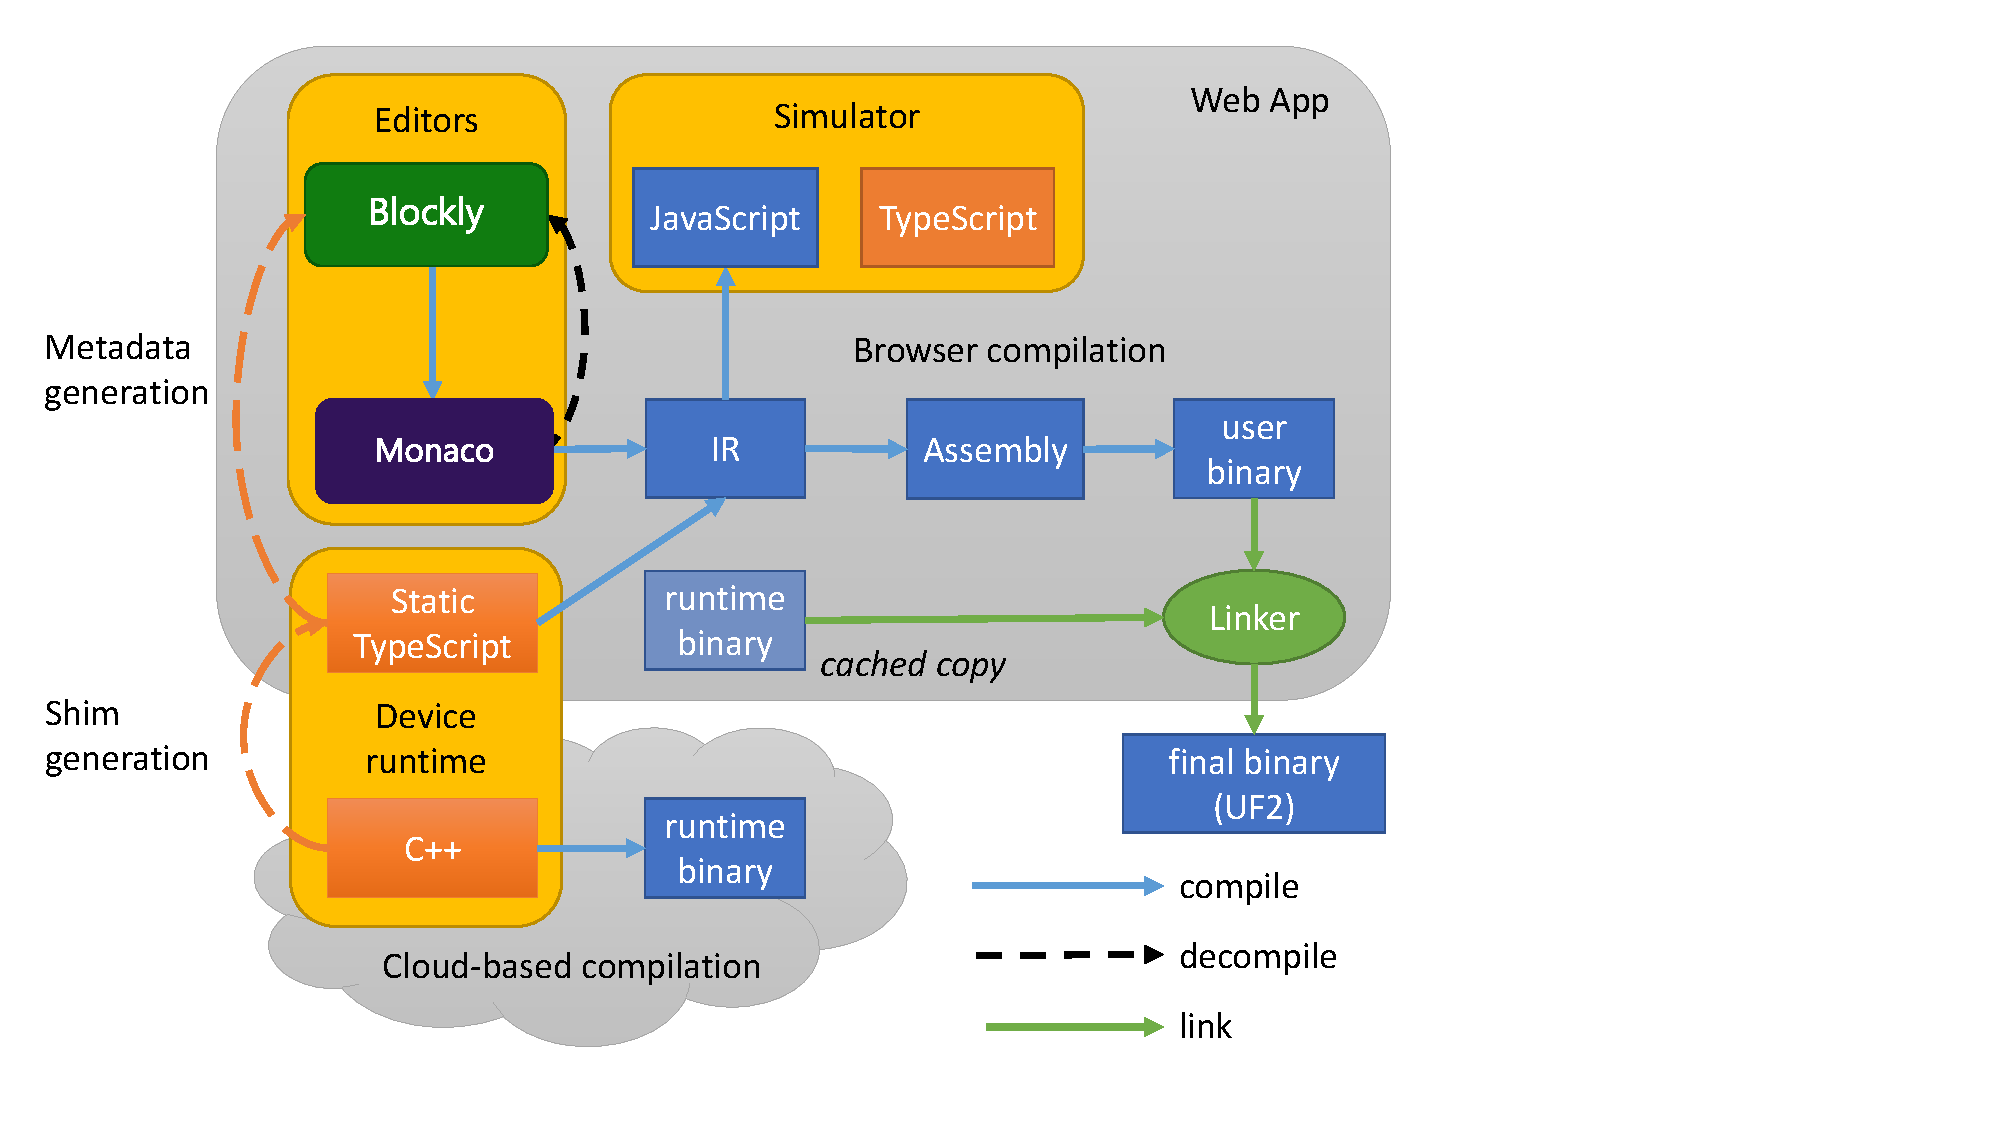
\includegraphics[width=5.5in]{makecodeFig.pdf}
\caption{\label{fig:makecode}\MC Architecture}
\end{figure*}

\subsection{Device Runtime and Shim Generation}

An \MC target is defined, in part, by its device runtime, which can be a combination of C++ 
and Static TypeScript (STS) code. The C++ runtime for the target microcontroller is precompiled 
and stored in the cloud. The runtime binary also is stored in the HTML5 application cache (with 
other assets) so that the web app can function when the browser is offline. Additional runtime
components may be authored in STS, which allows the device runtime to be updated without the
use of C++, and permits components of the device runtime to be shared by both the device
and simulator runtimes. The ability to author the device runtime in both STS and C++ is
a unique aspect of \MC's design.

Whether runtime components are authored in C++ or STS, all runtime APIs are exposed as fully-typed
TypeScript definitions, as described later. A full-typed runtime improves the end-user experience 
by making it easier to discover APIs; it also enables the type inference provided by the TypeScript 
compiler to infer types for (unannotated) user JavaScript programs.

\MC supports a simple foreign function interface from TypeScript to C++ based on namespaces,
enumerations, functions, and basic type mappings. \MC uses top-level namespaces (in both C++ and
TypeScript) to organize sets of related functions.  Preceding a C++ namespace, enumeration, or function
with \emph{//\%} indicates that \MC should map the C++ construct to TypeScript.
Within the \emph{//\%} comment, attributes are used to define the visual appearance for that
language construct, such as for the LED namespace in the micro:bit target:

\begin{lstlisting}
//% color=#5C2D91 weight=97 icon="\uf205"
namespace led { 
...
\end{lstlisting}

Figure~\ref{fig:screenSnap}(C) shows the toolbox of API and language categories, where the LED
namespace can been seen. Here is the C++ file defining the micro:bit's led namespace and its functions:
~\href{https://github.com/Microsoft/pxt-microbit/blob/master/libs/core/led.cpp}{pxt-microbit/libs/core/led.cpp}.

Mapping of functions and enumerations between C++ and TypeScript is straightforward
and performed automatically by \MC. 
Here's an example of the C++ function plot in the led namespace that wraps a more
complex function call of the underlying device runtime to set/plot an LED in the micro:bit display:

\begin{lstlisting}
//% blockId=device_plot block="plot|x %x|y %y"
//% x.min=0 x.max=4 y.min=0 y.max=4
void plot(int x, int y) {
    uBit.display.image.setPixelValue(x, y, 1);
}
\end{lstlisting}

We'll describe the attribute definitions in the \emph{//\%} comment in the next section. 
\MC uses a TypeScript declaration file to describe the TypeScript elements corresponding
to C++ namespaces, enumerations and functions.  We call such files shim files.
Since the C++ plot function is preceded by a \emph{//\%} comment, 
\MC adds the following TypeScript declaration to the shim file (shims.d.ts) and copies
over the attribute definitions in the comment. \MC also adds an attribute definition mapping
the TypeScript shim to its C++ function (shim=led::plot):

\begin{lstlisting}
//% blockId=device_plot block="plot|x %x|y %y
//% x.min=0 x.max=4 y.min=0 y.max=4 shim=led::plot
function plot(x: number, y: number): void;
\end{lstlisting}

Here is the shim file generated from C++ micro:bit device runtime:
\href{https://github.com/Microsoft/pxt-microbit/blob/master/libs/core/shims.d.ts}{pxt-microbit/libs/core/shims.d.ts}.

To support the foreign function interface, \MC defines a mapping between C++ and TypeScript types.
Boolean and void have straightforward mappings from C++ to TypeScript (bool $\rightarrow$ boolean, void $\rightarrow$ void). 
As JavaScript only supports number, which is a C++ float/double, \MC uses TypeScript's support
for type aliases to name the various C++ integer types commonly used for microcontroller programming
(int32, uint32, int16, uint16, int8, uint8). 
% don't use int, unsigned etc. they are actually different sizes on different compilers for AVR
This is particularly useful for saving space on 8-bit architectures such as the AVR. 

\MC allows a set of C++ functions with the same first parameter (of type Foo) to be
exposed as a TypeScript interface Foo as follows: this set of C++ functions must be grouped
inside a namespace of the name FooMethods.  See, for example, how a C++ buffer abstraction is exposed:
\href{https://github.com/Microsoft/pxt-microbit/blob/master/libs/core/buffer.cpp}{pxt-microbit/libs/core/buffer.cpp}.
You can find the resulting TypeScript Buffer interface in the previously referenced shim file for the micro:bit.

\MC includes reference counted C++ types for strings, lambdas (with
up to three arguments and a return type) and collections.  
\MC does not yet include garbage collection, so advanced users who create cyclic
data structures must be careful to break cycles in order to ensure complete deallocation. 

\subsection{Block Metadata Generation}

Both C++ and TypeScript APIs can be specially annotated (minimally via 
\emph{//\% block}) so that the \MC compiler generates the needed
Blockly metadata to expose an API as a visual block. So, to expose the previously
encountered plot function as a visual block (as well as a TypeScript function), one simply needs:
\begin{lstlisting}
//% block
void plot(int x, int y) { . . . }
\end{lstlisting}

Additional attribute definitions can provide text descriptions for the block, project function
parameters (thus simplifying the API available via Blockly), and describe other visual/functional
characteristics of the block.  \MC uses the types of function parameters to select appropriate
Blockly widgets.  For example, an enumeration is represented by a dropdown menu in blocks.
For more information on the block-specific annotations, see 
\url{https://makecode.com/defining-blocks}. 
\MC's support for Blockly means that for the common case, the target developer doesn't need
to know anything about the Blockly framework.  For more sophisticated needs, one can directly access
the Blockly framework. 

\subsection{Editors and Code Conversion}

\MC uses the Blockly (\emph{\href{https://github.com/google/blockly}{blockly}}) and Monaco 
(\emph{\href{https://github.com/Microsoft/monaco-editor}{monaco-editor}}) editors to allow the user to code with
visual blocks or TypeScript. The editing experience is parameterized by the full-typed device
runtime, which provides a set of categorized APIs to the end-user, based on namespaces, as
previously described. These APIs are visible in both editors via a toolbox to the immediate
left of the programming area. The Blockly and Monaco toolboxes show the same set of APIs, to
help in transition from coding with blocks to coding with JavaScript. More advanced TypeScript
APIs can be discovered in Monaco via code intellisense.

The Blockly program representation is compiled to Static TypeScript in a syntax-directed manner
(see \emph{\url{https://github.com/Microsoft/pxt/tree/master/pxtblocks}{pxtblocks}}). A key issue is the need for
type inference on the Blockly representation, as variables generally are defined and used without
being declared in Blockly. \MC uses a simple unification type inference to assign a
unique type to each variable.  
% this may not be possible:
%In the future, we expect to use TypeScript's type inference instead
%and eliminate the need for separate type inference over the Blockly representation. 
TypeScript supports programming constructs that are not available in Blockly, such as classes.
Such constructs are converted into grey uneditable blocks in Blockly, with the construct's program
text intact. This means \MC always can decompile a TypeScript program to Blockly and then recover
the program text of the grey blocks when converting from Blockly back to TypeScript
 (see \emph{\href{https://github.com/Microsoft/pxt/blob/master/pxtcompiler/emitter/decompiler.ts}{decompiler.ts}}). 

\subsection{Compilation Pipeline}

\MC first invokes the TypeScript language service to perform type inference and type checking on the 
user's program, using the TypeScript declaration files for the device runtime.   It then checks that the
user's program is within the STS subset through additional syntactic and type checks over the adorned
abstract syntax tree (AST) produced by the language service (detailed in Section XYZ).  Assuming all the
above checks pass, \MC then performs tree shaking and compilation of the AST of the user code and
device runtime to an intermediate representation (IR) that makes explicit: labelled control flow among a
sequence of instructions with conditional and unconditional jumps; heap cells; field accesses; store operations,
and reference counting.

There are four backends for code generation from the IR. The first backend simply generates JavaScript,
for execution against the simulator runtime.  A second backend generates assembler, parameterized by a
processor description.  Currently supported processors include ARM's Cortex class (Thumb instructions)
and Atmel's Atmega class (AVR instructions). A separate assembler, also parameterized by an instruction
encoder/decoder, generates machine code and resolves runtime references, producing a binary executable.
A third backend generates bytecode instructions and a fourth backend targets C\#. 
The compiler chain
can be found at \emph{\href{https://github.com/Microsoft/pxt/tree/master/pxtcompiler/emitter}{pxtcompiler/emitter}} and 
\emph{\href{https://github.com/Microsoft/pxt/tree/master/pxtlib/emitter}{pxtlib/emitter}}.


\subsubsection{Asynchronous Functions}

An important part of the compilation process is to allow users to call asynchronous 
TypeScript functions (identified through the \emph{//\% async} annotation) 
as if they were blocking functions.  
For execution in the browser,
every function is compiled so that it can be suspended (at the return of a call) and later resumed (at the same point). 
The default behavior at a suspension point is to immediately resume execution.  For a call to an async function,
the default behavior is overridden by the compiler, which suspends execution of the current function. 
Upon completion of the async function call, the current function then is resumed. Such async functions are written
by runtime developers, not end-users, and greatly simplify the JavaScript
programming model for end-users. For example, although the JavaScript simulator runtime uses promises to 
achieve asynchronous execution in a single-threaded context, these promises are hidden from the end user. 
The CODAL device runtime supports fibers with the ability to pause, so for compilation to a device, 
the compiler simply emits a call to pause at a suspension point. 

\emph{TODO: need a small example to clarify how it all works}

% tball: I added TypeScript above to make it clear 
%\emph{TODO: The async annotation is only relevant for the JS code. In ARM/AVR it doesn't do anything.
%One way to say it is to say it's there to simulate cooperative multi-threading in JS, since
%it is already implemented in C++ by CODAL.}

\subsubsection{Untagged and Tagged Strategies}

The \MC compiler supports the Static TypeScript language subset described in Section~\ref{sec:sts},
with two compilation strategies: untagged and tagged. Under the untagged strategy,
a JavaScript number is interpreted as a C++ int by default and the type system is used
to statically distinguish primitive values from boxed values. As a result, the untagged
strategy is not fully faithful to JavaScript semantics: there is no support for floating
point and the Null and Undefined types are represented by the default integer value of zero.
This strategy is used for the micro:bit and Arduino Uno targets. 

In the tagged strategy, numbers are either tagged 31-bit signed integers, or if they do not fit, 
boxed doubles. Special constants like false, null and undefined are given special values 
and can be distinguished. The tagged execution strategy has the capability to fully support
JavaScript semantics. This strategy is used for all SAMD21 targets.

\subsection{Simulator}

A \MC target can provide an alternate TypeScript implementation for each API in the device runtime, for use in the device
simulator. As this code runs in the web browser (not on the actual device) and manipulates the DOM, the developer is free to
use all of TypeScript/JavaScript's features. (As an aside, \MC also support ``simulator-only'' targets that have no 
associated device; in these cases, the ``device runtime'' is defined solely by the simulator APIs.) 

The simulator allows the user to experience the basic functions of the device in the browser and to test their code
before deploying it to the actual device. The simulator has proxy widgets for sensors such as accelerometer (mouse motion),
temperature and light, allowing the user to control the sensor's value.  The simulator only provides basic functionality
and is far from a complete device emulation.   For example, it is not possible for the user to simultaneously modify two
inputs to the simulated device, while it is possible with the actual device (i.e., shaking it to change the accelerometer
reading while pushing one of the device's buttons).

%\MC provides various components to make device simulators easier to build: board, parts, wiring, etc.

\subsection{Packages and Custom Editors}

Packages are \MC's dynamic/static library mechanism for extending a target (by adding new code/data to the device
and simulator runtimes, as well as accompanying documentation). The following package extends the micro:bit target so
that the micro:bit can drive a NeoPixel strip of RGB LEDs: \url{https://github.com/Microsoft/pxt-neopixel}. 

To see how this
package is surfaced to the end-user, visit \url{http://makecode.microbit.org/} and select the ``Add Package'' option from the
gear menu; you will see the package ``neopixel'' listed in the available options. If you click on it, a new block category
named ``Neopixel'' will be added to the editor. In this scenario, PXT dynamically loads the (white listed) neopixel 
package directly from GitHub, compiles it and incorporates it into the web app. Packages also can be bundled with a web
app (the analog of static linking).  

For packages containing C++ files, a new C++ runtime has to be compiled in the cloud.
This is achieved by collecting all C++ files (in all packages plus the CODAL runtime),
computing a hash, checking in the local in-browser cache if such a runtime was retrieved
before, and otherwise asking the cloud service to compile it.
Of course, the cloud service will return a cached copy, if the same set of C++
files was compiled before. The cache hit rates, in both the browser cache
and the cloud cache, are very high. 
The first hit rate is high because the cloud needs to be consulted
only when a new package is added to the project, and this particular combination 
of packages was never used before on current machine.
The second hit rate is high because people rarely combine many packages (due to
hardware and memory constraints), and there are only so many of them.

    \section{Static TypeScript}
\label{sec:sts}

TypeScript is a typed superset of JavaScript designed to enable JavaScript developers to take advantage of code 
intellisense, static checking and refactoring made possible by types (\url{http://www.typescriptlang.org/}). 
As a starting point, every JavaScript program is a TypeScript program.  Types can be added gradually to such programs, 
supported by type inference. In TypeScript, the Any type 
represents any JavaScript value with no constraints. Type inference may assign the Any type to expressions for which 
no more specific type can be inferred.

While TypeScript provides classes and interfaces with syntax like Java/C\#, their semantics
are quite different, as they are based on JavaScript.  Classes are simply syntactic sugar for creating objects that
have code associated with them, but these objects are JavaScript objects with all their dynamic semantics intact. This
is not surprising, as TypeScript was designed to accommodate the dynamic nature of JavaScript and programming patterns
familiar to the JavaScript programmer. 

We approach TypeScript from the viewpoint of the microcontroller programmer, who is 
familiar with the static (though unsound) type systems of C and C++. Our realization is that TypeScript contains a
statically-typed sound subset (Static TypeScript: STS, for short) that closely resembles Java and C\# in its semantics.
STS arises from TypeScript by:
\begin{itemize}
\item \emph{eliminating} the Any type from the type system, as well as JavaScript statements
and expressions that only can be typed with Any;
\item \emph{partitioning} TypeScript's space of object types into functions, records, constructor functions, and arrays, with no casts 
    possible between the partitions (and eliminating all other object types) - structural subtyping is used to relate records 
    to each other, as in TypeScript;
\item typing of classes \emph{nominally} rather than structurally, as in TypeScript, and traditional function subtyping (contravariant 
    in the argument type, covariant in the return type) for functions as well as methods;
\item \emph{restricting} casts between records and classes: a class can be cast to a record, but a record cannot be cast to a class.
\end{itemize}
STS is a syntactic subset of TypeScript -- there is no change to the syntax of TypeScript.
In terms of type checking, STS also is a subset of TypeScript. Simply put, given a STS program $P$,
for every type compatibility or subtype relation $R(P)$ of TypeScript, the corresponding relation $R'(P)$ in STS
is a subset of relation $R$. Every STS program is a TypeScript program. 

STS guarantees the absence of runtime type errors, including downcasts.
The major class of runtime errors still possible is dereference of null/undefined values. 
STS can be supported by a simple runtime model, like that for C++, using classic vtables and interface tables,
rather than the prototype-based runtime model used for JavaScript.

\subsection{Eliminating Types: Any, Union, Intersection}

By default, the TypeScript compiler assigns the Any type to an expression/declaration for which it is unable to 
infer a more precise type. STS uses the \emph{--noImplicitAny} option to direct the TypeScript compiler to raise an error 
whenever it makes an (implicit) assignment of the Any type.  STS also checks for an explicit use of the Any type in
the program and raises an error. Many JavaScript constructs can only be typed with the Any type, including: prototype lookup,
the \emph{eval} and \emph{with} statements, a \emph{this} reference outside of class context, an index access on non-array object, and
reflection on Function/Object objects. Therefore, these constructs are not in STS. For good measure,
STS also excludes TypeScript's union and intersection types.

\subsection{Partitioning of Object Types}

In TypeScript, object types are used to describe dictionaries, functions, arrays, class instances,
as well as objects that take on multiple of the above roles, as is common in JavaScript. Object types are
related to one another by structural subtyping.  Interface declarations name object types; classes add implementation
and the ability to statically inherit implementation from super classes. Per the TypeScript specification~\cite{TSspec2016}:
\begin{itemize}
\item ``object types are composed from properties, call signatures, construct signatures, and index signatures, collectively called members'';
\item ``interfaces provide the ability to name and parameterize object types and to compose existing named object types into new ones.''.
\end{itemize} 
Object types and the interface declarations that describe them enable the typing of a JavaScript object that plays multiple roles
(as a function, dictionary, etc.). For example, here is an interface that describes an object that is a function from number to number
and also has property (foo) which is a string:
\begin{lstlisting}
interface Bar {
    (x: number): number; // call signature member
    foo: string;         // property member
}
\end{lstlisting}
STS partitions the space of object types as follows:
\begin{itemize}
\item[1.] a \emph{record} type has only (member) properties;
\item[2.] a \emph{function} type has exactly one member, a call signature;
\item[3.] a \emph{constructor function} type: has at least one constructor signature and no other signature kind;
\item[4.] an \emph{array} type has a numeric index signature and no other signatures;
\item[5.] an \emph{other} type: object type not covered by the previous four categories.
\end{itemize}
STS excludes all ``other'' types, leaving us with the four kinds of types.
The partitioning is further reflected in STS's subtype relation: 
types $T$ and $U$ from different partitions (in the first four partitions above)
are not related by STS's subtype relation.

\subsection{Treatment of Classes and Methods}

TypeScript introduces two (object) types for each class declaration:
\begin{itemize}
\item a constructor function type by which instances of a class
are created (and static properties accessed), as seen in the previous section; 
\item a class type describing the instances of the class, which is a record type, but
with public/private/protected modifiers on its properties (in a record type, all properties are public).
\end{itemize}
TypeScript's treatment of class types as record types
means that it is possible to assign to a property representing a method, 
destroying the class abstraction that ties together code and data. This also 
eliminates the possibility of using a shared vtable implementation for classes.

STS adds a new partition to represent class types, separate from record types, describing the instances of classes.
Classic nominal subtyping is applied to class types, with function subtyping used to relate methods with 
the same name in subclass and superclass, per TypeScript, just as record types are treated.
Furthermore, STS permits a cast from a class type
to a record supertype, but does not allow any casts from record types to class types. This means
it is possible to use interfaces to abstract over classes, as in Java and C\#. 

Finally, STS enforces that a function may not be assigned to a property of a record type, 
though it is possible to construct records with function properties using object literals. 

\subsection{Subtyping and Type Checking}

In STS, $S$ is a subtype of a type $T$ if one of the following is true:
\begin{itemize}
\item $S$ and $T$ are identical types;
\item $S$ is the Undefined type;
\item $S$ is the Null type and $T$ is not the Undefined type;
\item $S$ is an enum type and $T$ is the primitive type Number;
\item $S$ is a string literal type and $T$ is the primitive type String;
\item $S$ and $T$ are class types and all the following are true:
\begin{itemize}
  \item $S$ is derived from $T$ (via \emph{extends} clauses);
  \item checkProps($S$,$T$) holds;
\end{itemize}
\item $S$ is a class/record type and $T$ is a record type and
\begin{itemize}
  \item checkProps($S$,$T$) holds;
\end{itemize}
\item $S$ and $T$ are function types such that all the following hold:
\begin{itemize}
  \item $S$ has at least as many parameters as $T$;
  \item each parameter type in $T$ is a subtype of the corresponding parameter type in $S$;
  \item the result type of $T$ is Void, or the result type of $S$ is a subtype of that of $T$;
\end{itemize}
\item $S$ and $T$ are array types and all the following hold:
\begin{itemize}
\item $T$ has a numeric index signature with element type $U$, 
    and $S$ has a numeric index signature with element type $V$
    such that $V$ is a subtype of $U$;
\item checkProps($S$,$T$) holds.
\end{itemize}
\end{itemize}

% https://www.earthli.com/news/view_article.php?id=3391

Given types $S$ and $T$, checkProps($S$,$T$) holds if for each property $N$ in $T$, 
$S$ has a property $M$ where all of the following are true:
\begin{itemize}
\item $M$ and $N$ have the same name;
\item the type of $M$ is a subtype of the type of $N$;
\item $M$ and $N$ are both public, or $M$ and $N$ are both 
      private (protected) and originate in the same declaration, 
      or $N$ is protected and $S$ is a class derived from class $T$
\end{itemize}

STS type checking for (pure) expressions remains the same as in TypeScript.
Type checking at assignments, where a value of type $S$ flows (is assigned to) 
into a location of type $T$ uses the new subtyping relation: $S$
must be a subtype of $T$.  Downcasts (where a supertype flows to a subtype)
are not permitted in STS.

    \begin{figure}[t]
    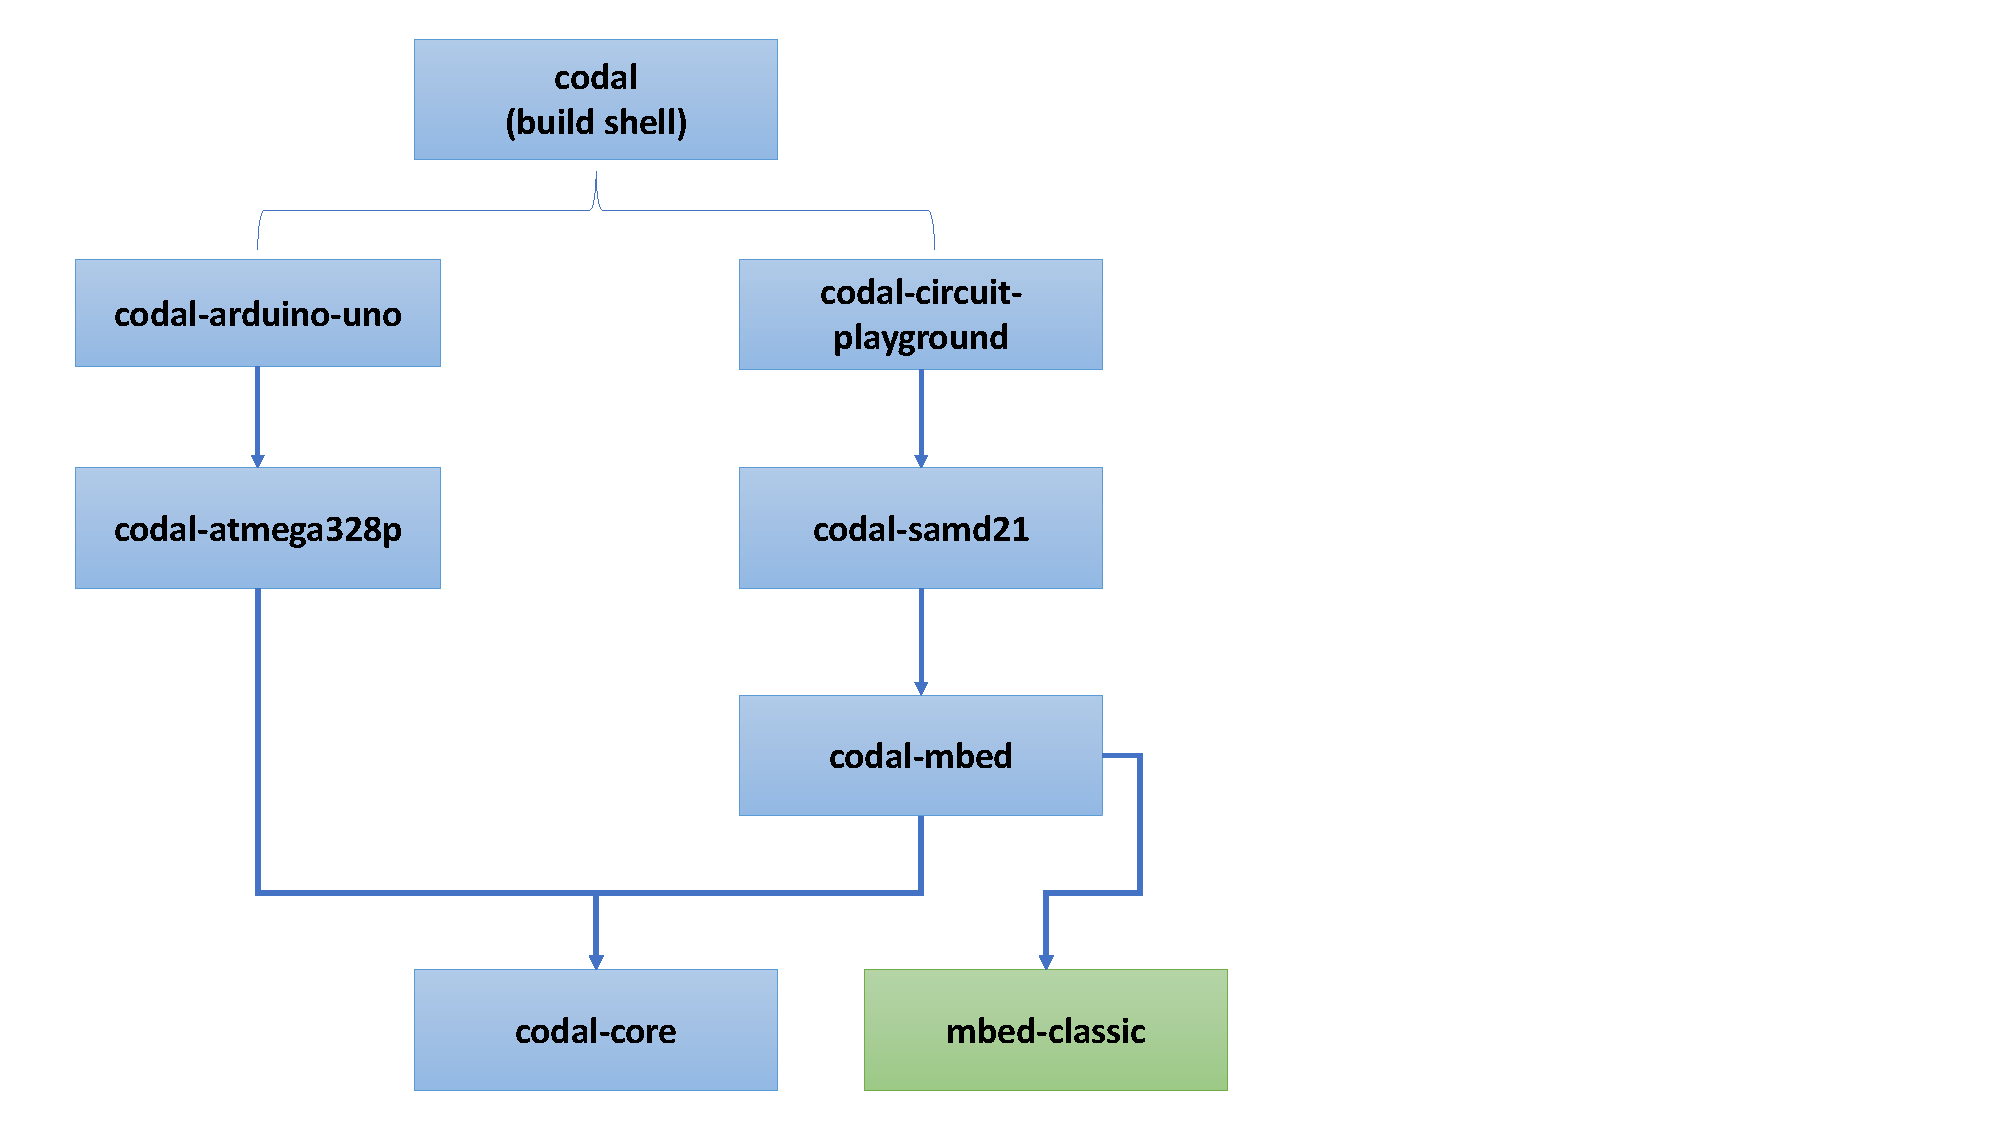
\includegraphics[width=4.5in]{codalFig.pdf}
    \caption{\label{fig:codal}Detailed relationships between \CO repos.}
\end{figure}

\section{The \CO Runtime}
\label{sec:codal}

The component-oriented device abstraction layer (\CO) is a multi-platform runtime designed to make efficient use of memory and energy, provide both synchronous and asynchronous API variants, and be a reasonable target for higher level languages such as JavaScript.

\CO provides a set of components that abstract away microcontroller specifics, a non-preemptive scheduler that minimises the need for resource locking primitives whilst allowing asynchronous operation, and an eventing subsystem (common to all components) that enables the decoupling of system and user code.

\CO components represent software or hardware drivers (e.g., an I2C device, a GPIO pin, a Message Bus, a Bluetooth device); any component can generate or consume events. \CO supports both polling and asynchronous (event-driven) programming models, which enables higher level languages to map straight onto native C/C++ APIs. Section~\ref{sec:related} compares \CO to other runtimes and operating systems for microcontrollers.

% more required here, needs to be reflowed...

\subsection{Structural Overview}

\begin{figure}
% TODO: shrink width
\begin{lstlisting}
class ArduinoUno : public CodalDevice
{
    ...
    public:
        ATMegaTime       timer;
        ATMegaSerial     serial;
        ArduinoIO        io;
        ATMegaI2C        i2c;
        MessageBus       messageBus;

        ArduinoUno();
};
\end{lstlisting}
\caption{\label{fig:codalSingleton}Singleton for Arduino Uno}
\end{figure}

Figure~\ref{fig:codal} shows the repository architecture for two \CO devices, the Adafruit CircuitPlayground, built on top of ARM's mbed, and the Arduino Uno, built without any supporting libraries. The \COLN-core repo sits at the base of both device trees and provides the high level driver models which are implemented in the layer above. Each target library (\COLN-arduino-uno, \COLN-circuit-playground) builds on top of a processor library containing processor specific files, and the target library at the top of the tree contains files specific to a device --- commonly the linker script and the model for a device. A model is a C++ class that brings together components defined further down the tree as a single software representation of the device,
as shown in Figure~\ref{fig:codalSingleton}.
This architecture enables platform independent code to run across multiple processors and devices, while allow for extensibility and specialisation.

\subsection{Message Bus and Events}

Message passing via events is a common technique and is the foundation of many operating systems --- yet in most systems events are static, used only to notify users of key events within the system (e.g. SIGKILL on UNIX).


\CO offers extensible events where the data contained in an event can be arbitrary, and application specific. Application developers can then ``listen'' to events, specifying an id (namespace), a value (unique within a namespace), and a function to be invoked when an event is raised. All events pass through the message bus: if a corresponding listener is in place, the function indicated by the listener is invoked. The eventing model aligns well to JavaScript and languages with event-based programming models.

Not only do events enable easy modularisation of code, but they also safeguard the application programmer from situations where incorrect code could cause unexpected behaviour. Take for example an application to detect a button press, there are usually two solutions: (1) poll the state of a pin; or (2) configure an interrupt to fire when the state of a pin changes.

\begin{figure}
\begin{lstlisting}
int state = 0;

void buttonClicked() {
    int gpioState = PIN0;
    // button released, blink LED!
    if(state == 1 && gpioState == 0) {
        set_state(LED, 1);
        wait_ms(1000);
        set_state(LED, 0);
    }
    state = gpioState;
}

int main() {
    configure_interrupt(PIN0, buttonClicked);
    while(1);
}
\end{lstlisting}
\caption{\label{fig:pollPin}Pseudocode for detecting a pin transition (polling).}
\end{figure}

Figure~\ref{fig:pollPin} shows an example of polling.
  This code is considered bad practice as it prevents other interrupts (like Timers) from firing for at least a second when a button is released, however, this is often the first application that a user will create. Such frameworks advise users to avoid blocking functions and waiting in interrupt context, thus sidestepping the problem by punting responsibility to the user --- \CO uses the message bus abstraction to shield users from such scenarios, as shown in Figure~\ref{fig:messageBus}. Note that the user doesn't have to configure any interrupts, as they are handled by pre-existing drivers.

\begin{figure}
\begin{lstlisting}
#include "CircuitPlayground.h"
CircuitPlayground cplay;

void buttonClicked() {
    cplay.io.led.setDigitalValue(1);
    cplay.sleep(1000);
    cplay.io.led.setDigitalValue(0);
}

int main() {
    cplay.messageBus.listen(ID_BUTTON_A,DEVICE_BUTTON_EVT_CLICK,buttonClicked);

    while(1) cplay.sleep(100);
}
\end{lstlisting}
\caption{\label{fig:messageBus}Using the message bus.}
\end{figure}


% Stuff to add (it's already quite long):
% * Provides a similar mechanism seen in higher level languages
% * Timer and queues?
% * message passing microkernel

\subsection{Fiber Scheduler}

Novice users often want to perform multiple operations concurrently, generally requiring threads. \flameon{TBALL: I don't think that it's that they `want` to do it - it's more that the event-based paradigm leads naturally to concurrency, especially in a reactive setting, like that of the microcontroller.}
Threading is a confusing concept: users have to learn about locks, semaphores, and preemption, to prevent race conditions. Threads can also consume a large number of resources depending on the model that is adopted by the runtime environment.

\CO takes a non-preemptive scheduling approach which reduces the need for resource locking primitives. \CO fibers (lightweight threads) are RAM efficient and have a variable stack size. As we adopt a non-preemptive scheduling model, user or driver code must call ``sleep'' to swap context to another fiber, this means that at an invoke of sleep, the stack depth is small. When a fiber is paged out the entire stack is duplicated to the heap. This would normally be ill-advised, but due to a usually small stack size, this is more efficient than approaches where there is a mandated stack size.

Events and the message bus are integral to \CON, even extending to fibers, which can block and wait on events to complete. \flameon{TBALL: this is not much of a sentence - please revise.}

\subsection{Drivers}

Drivers are commonly programmed via low-level interfaces that control external or integrated hardware on a device. For embedded developers, creating and using drivers involves translating datasheets into program code and using such interfaces, which can confuse novice programmers.

\CO drivers abstract away the complexities of the underlying hardware into reusable, extensible, easy-to-use components: for every hardware component there is a software component. \CO has three types of drivers:
\begin{itemize}
    \item[1.] an abstract specification of a driver model common to most devices (e.g. I2C, Serial);
    \item[2.] a driver that relies only on the interfaces specified in a driver model  (e.g. an I2C based driver);
    \item[3.] the concrete implementation of the abstract driver model, which may be platform specific or platform agnostic.
\end{itemize}
Not all devices are the same, and by generalising the interface, devices can introduce platform specific optimisations and specialisations.

Interrupts are integral to drivers: in serial communications it is useful to know when a byte has been sent or received. As illustrated in the button example, performing operations in interrupt context can be detrimental to the device. \CO drivers use events to decouple computational tasks, that may take a variable length of time, from interrupt context.

% * motivation
% * example - I2C, microphone (DMA)
% * one component per piece of hardware or software
% * Provides a common interface
% * uses events to decouple from interrupt context.

\subsection{Memory Management}

Standard libraries in C++ do not offer reentrant versions of memory allocation calls like ``malloc'' and ``new'', forbidding the allocation of memory in interrupt context.

\CO implements its own heap allocater that is designed to safeguard users from the scenario above, introducing reentrant versions of malloc. The heap allocater is flexible, reconfigurable, and repurposable, allowing the specification of multiple heaps across memory and it is optimised for common sizes and repeat allocations.

\CO has a number of managed types that use reference counting to determine when memory should be freed. Internally, managed types use malloc to copy stack allocated data to the heap creating a safer environment for the user --- the reentrant behaviour of malloc and free are key here, as references can be created and destroyed regardless of processor context.
% * provides an interrupt safe environment for memory allocation
% * flexible implementation
%     - multiple heaps
%     - reconfigurable, repurposeable
% * optimisations for common sizes and repeated patterns
% * edu
% * couple of sentences on types
%     - ref counted, malloced types.

\begin{figure}
\begin{lstlisting}
CircuitPlayground cplay;
SAMD21DMAC dmac;
Synthesizer synth;
SAMD21DAC dac(cplay.io.speaker, dmac, synth.output, 44100);

int main()
{
    // Align sample rate to speaker DAC.
    synth.setSampleRate(dac.getSampleRate());
    synth.setTone(Synthesizer::SawtoothTone);
    synth.setFrequency(300);

    while(1) cplay.sleep(100);
}
\end{lstlisting}
\caption{\label{fig:play}Playing a tone using Streams.}
\end{figure}

\subsection{Streams}
There are very few scenarios where a processor alone is used to accomplish a task, hence the growth in packaged devices where sensors are distributed alongside a main processing unit. With sensors on boarded, scenarios are centered on the processing, handling, and piping of information generated by sensors.

One scenario is the generation of audio data for a speaker, which has a specific clock rate at which buffers are consumed. Rate pacing the passing of audio buffers to the speaker is challenging --- should it be the users' responsibility to ensure buffers are delivered at the correct time?

In \CON, a stream interface removes the complexity of these scenarios from user applications. Streams are formed of one source node (where data is generated), one sink node (where data is consumed), and 0 or more intermediate data streams which have knowledge of both upstream and downstream interfaces, forming a chain of filters and/or data processing units. Source nodes can push data into the stream, a sink node can pull data down the stream, and a data stream can do either (a Pull/Push model). This means that autonomous tasks can happen in the background, only requiring user intervention if the user application demands it.

The code in Figure~\ref{fig:play} will play a SawtoothTone whilst the device is powered on.

    \section{USB Flashing Format}
\label{sec:uf2}

The way that code gets from a host computer onto a microcontroller is deeply rooted in 1980's technologies - 
serial wires, obscure protocols, and text based file formats with limited line length. Depending on exact circumstances,
one must install serial USB drivers, select the right port and parameters, and then use a native application to access
the microcontroller. As the advance of maker content in educational curricula continues,
this complicated flashing process presents one of the major obstacles to adoption in schools, 
where installing any software is usually the domain of IT administrators.

One solution would be to rely on emerging standards, like WebUSB and WebBluetooth to transfer a program from the browser 
to the microcontroller. These standards are however still in their infancy, and it may take even longer before they are 
deployed in schools.

Another solution was pioneered by ARM with its DAPLink firmware, where a USB-capable microcontroller presents itself 
to an external computer as a USB pen drive. No special drivers need to be installed, as operating systems support pen
drives out of the box, typically formatted using FAT. The USB pen drive protocol (Mass Storage Class or MSC) is a
block-level protocol (generally 512 bytes) with no concept of files. DAPLink exposes a virtual FAT file system, which
is very small and never changes due to OS writes - it has an informational text file and an HTML file with a redirect
to the online editing environment. Otherwise, the FAT and the root directory table are empty. When the OS tries to
read a block, the DAPLink computes what should be there, based on compiled-in contents of the info and HTML files.
On file system writes, DAPLink detects the Intel HEX format~\cite{IntelHEX}, 
decodes it and flashes the file's contents into the target microcontroller's memory. 

Let's consider the problem that DAPLink must solve: it sees a 512 byte block of data to be written
at a particular block index on the device and must decide if it's part of the file being flashed and, if so, extract
the data and write it to the target microcontroller. Furthermore, when the OS writes a HEX file, DAPLink needs to discard
writes to the FAT or directory table, as well as writes of the meta-data files. It may need to deal with out-of-order writes.
All these details mean that DAPLink is quite complex and sometimes needs to be updated when a new OS release changes the way
in which it handles FAT. This also is the reason that some MSC bootloaders for various chips only support given operating
systems under specific conditions.

The task would be simplified then, if every 512 block of the file being flashed was easy to distinguish from meta-data
or other random files, and easy to act on, independent of other blocks. Intel's HEX file format doesn't give us these properties 
- the 512 byte boundary can be in the middle of a line in the HEX file, and even if we have an entire line, every line only
contains the last 16 bits of the address where to flash, with the upper 16 supplied only when they change.

For these reasons, we designed the USB Flashing Format (UF2). It consists of 512 byte blocks, where each block contains:
\begin{itemize}
\item magic numbers at the beginning and end (to heuristically distinguish it from any other data the OS writes);
\item the address in the target chip flash memory where the payload should be written;
\item the payload data (up to 476 bytes)
\end{itemize}

% A UF2 file consists of 512 byte blocks. Each block starts with a 32 byte header, followed by data, and a final magic number. All fields, except for data, are 32 bit unsigned little endian integers.

% Offset	Size	Value
% 0	4	First magic number, 0x0A324655 ("UF2\n")
% 4	4	Second magic number, 0x9E5D5157
% 8	4	Flags
% 12	4	Address in flash where the data should be written
% 16	4	Number of bytes used in data (often 256)
% 20	4	Sequential block number; starts at 0
% 24	4	Total number of blocks in file
% 28	4	File size or reserved (write as zero)
% 32	476	Data, padded with zeros
% 508	4	Final magic number, 0x0AB16F30

The file format is designed specifically to deal with the following problems:

\begin{itemize}
\item operating system (OS) writing blocks in different order than occurs in a file;
\item OS writing blocks multiple times;
\item OS writing data that is not a UF2 block;
\item OS writing first/final part of a block, possibly for metadata detection or search indexing;
\end{itemize}

The magic number at the end helps to mitigate partial block writes.
Second and final magic numbers were randomly selected, 
except for the last byte of final magic number, which was forced to be `\\n' (0xA). 
Together with the first magic number being ``UF2\\n'' this makes it easy to identify UF2 blocks in a text editor.


The header is padded to 32 bytes, as hex editors commonly use 16 or 32 bytes as line length. 
This way, the data payload is aligned to line start.

32 bit integers are used for all fields so that large flash sizes can be supported in future, as well as for simplicity.
Little endian is used, as most microcontrollers are little endian. 8 bit microcontrollers can choose to just use the
first 16 bits of various header fields.

The total number of blocks in the file and the sequential block number make it easy 
bootloaders to detect that all blocks have been transferred. It requires one bit of 
memory per block (eg., on SAMD21G18A it's 128 bytes). Alternatively, the bootloader might
ignore that and just implement a reset after say 1 second break in incoming UF2 blocks.

The only file system assumption we make is that blocks of file are aligned with blocks on the hard drive. 
It's likely true of many file systems besides FAT. We also assume that USB MSC device reports its block 
size to be a multiple of 512 bytes. In the wild these devices always almost report exactly 512, and some 
operating systems do not support other values.

\subsection{Overheads}

Target chips usually can only write their flash in chunks larger than page size. On the SAMD21, pages are 64 bytes 
but need to be erased four pages at once, so the effective page size is 256 bytes. Therefore, UF2 for SAMD21 uses 
only 256 out of the 476 byte payload, so every block can written to flash straight away. This is still more 
efficient than HEX (which stores every byte as two ASCII characters and adds 20-30\% overhead). It also doesn’t 
matter - the file is transferred at USB full speed (around 1MB per second), and so the limiting factor is writing 
to flash.

Each block also can contain an optional total number of blocks in the file and the current block number. 
This lets the bootloader detect the end of the transfer (by keeping bitmap of all written blocks, 
as we assume blocks can be written more than once).



    \section{Evaluation}
\label{sec:evaluate}

\MC and \CO have been actively deployed for over a year, and bring the benefits of a 
high level type safe event based languages to thousands of active users. 
In this section we provide a broad, quantitative evalaution of the cost at which 
these benefits are realised. We do this through the generation of a number of micro 
benchmarks that give insights into the performance of \MC and \CO on a selection of 
physical devices. 

The support software of our platform consists of two essential layers. Throughout this
section we break down results into these layers to give an insight into how each layer performs.
(we refer to \emph{\MC wrappers} as \MC throughout this evaluation):

\begin{itemize}
\item \emph{\CO}: the device runtime, against which we write C++ programs;
\item \emph{\MC wrappers}: the C++ and Static TypeScript wrapping for \CO
to make it known to \MC, against which we write Static TypeScript programs;
\end{itemize}

\subsection{Methodology}

To analyse the performance of our solution, we have written a suite of programs to evaluate 
different aspects of \MC and \CO when running on a representative selection of real hardware devices. 
Throughtout, we use the native C++ benchamarks provided by \CO as a baseline, and the Static TypeScript benchmarks show the overhead
added by \MC. 

These programs were written in both C++ and Static TypeScript, and evaluated on the three microcontrollers 
listed in (Table~\ref{table:devices}): The Nordic nRF51 based micro:bit, the Atmel SAMD21 based CPX, and the Atmel Atmega (Uno). 

The Uno is the simplest of these devices, consisting of an 8-bit processor running at 48 MHz, 
it only has 2kB of RAM and 32kB of flash. 
The Uno has no onboard components other than the microcontroller which supports 
GPIO, Serial, and I2C.

The micro:bit has a 32-bit Cortex M0 clocked at 16MHz, with 16kB RAM and 256kB of flash. It has a number of onboard components 
including a 5x5 LED matrix display, a compass, accelerometer, buttons, GPIO, I2C, Serial, and Bluetooth Low Energy.

The CPX is a 32-bit Cortex-M0+, which offers greater energy efficiency and performance; it clocks at 48 MHz, has 32kB of RAM and 
256kB of flash. On board the CPX are: RGB pixels, an infrared transmitter and receiver, a touch sensor, buttons, accelerometer, speaker, 
microphone, GPIO, I2C, and Serial.

The Uno and micro:bit \MC targets use the untagged strategy, while the CPX target takes the tagged strategy (see Section~\ref{sec:untagged-tagged}).

Our benchmarks are be classified into two types, each with their own methodology:

\begin{enumerate}
    \item \textit{Performance Analysis}: Tests that capture time taken to perform a given operation. here we instrument
    \MC and \CO to perform toggle physical pins on the device at key points in the test code. We them measure the time to
   execute the operation, by using a calibrated oscilloscope observing these pins. This allows us to derive highly accurate real time 
   measurements without biasing the experiment.

    \item \textit{Memory Analysis}: Tests that capture the RAM or FLASH footprint of a certain operation will log a map of memory 
    before executing the operation, execute the operation, and log a map of memory at the end of the operation. 
    A serial terminal is then used to capture the output of these tests.
\end{enumerate}

It is important to note that memory and performance analysis are done in separate runs, 
to ensure logging does not affect time-related measurements.

\subsection{Tight Loop Performance}

To place the performance of \MC in context, we perform a comparative evaluation of \MC against two state-of-the-art 
solutions, using the native C++ as our baseline. The two points of comparison are MicroPython~\cite{MicroPython}, an implementation 
of Python for microcontrollers, and Espruino~\cite{espruinoBook}, an implementation of JavaScript for micrcontrollers. 
For the CPX, a fork of MicroPython known as 'CircuitPython' was used. Both MicroPython and Espruino adopt virtual machine based
approaches.

To give an indicative general case execution time cost of each solution, we created a simple program that simply 
counts for 0..100000 in a tight loop in each solutions' respective language; 
the results are shown in Table~\ref{table:vm-comparison}. 
On AVR we only count to 25000, to fit in the 16 bit \texttt{int}, and scale up the results.

For the micro:bit, MicroPython and Espruino are \emph{two or more orders of magnitude slower} than a native \CO program. 
\MC performs only 2x slower. The slowdown reflects the simplicity of the STS compiler.
It should be noted that \MC for the CPX uses the tagged approach, which allows for seamless runtime switching to floating point numbers,
resulting in a further 3x slowdown. For both devices, we can observe that \MC outperforms both the VM-based solutions of MicroPython and 
Espruino by at least an order of magnitude. 

MicroPython and similar environment do not run on Arduino Uno due to flash and RAM size limitations.
We have also run into these, and as a result developed two compilation modes for AVR.
One compiles STS to AVR machine code, and the other (\MC VM) generates density-optimized byte code for 
tiny (around 500 bytes of code) interpreter.
The native strategy achieves code density of about 60.8 bytes per statement,
which translates into space for 150 lines of user code.
The VM achieves 12.3 bytes per statement allowing for about 800 lines.
For comparison, the ARM Thumb code generator used in other targets achieves
37.5 bytes per statement, but due to the larger flash sizes we did not run
into space issues.

% Since the Uno is an extremely resource constrained device, the AVR VM was specifically designed for high code density. The interpreter is implemented in assembly, always included with the program, and is around 0.5k. There are about 30 opcodes, some of which can take 1 or 2 byte arguments. There are also a few combined opcodes, representing a sequence of one argument-less opcode, and one with an argument, which improves code density by about 25\%. Opcodes are direct offsets into the code of the interpreter, speeding up execution. They operate on a stack (mainly for function calls) and a special scratch register. There is essentially no stack space overhead compared to native AVR compilation. The speed overhead is around 4x-5x (with respect to native) for computational tasks.

MicroPython and Espruino currently require more RAM and FLASH resource than is available in this device.

\begin{table}[]
    \centering
    
    \begin{tabular}{c|c|c|c|}
    \cline{2-4}
    \multicolumn{1}{l|}{}             & UNO    & micro:bit & CPX   \\ \cline{1-4}
    \multicolumn{1}{|c|}{\CO}         & 171ms  & 102ms     & 31ms  \\ \hline
    \multicolumn{1}{|c|}{\MC}         & 2.4x   & 2.1x      & 7.3x  \\ \hline
    \multicolumn{1}{|c|}{\MC VM}      & 15.3x  & -         & -     \\ \hline
    \multicolumn{1}{|c|}{MicroPython} & -      & 98x       & 183x  \\ \hline
    \multicolumn{1}{|c|}{Espruino}    & -      & 1133x     & -     \\ \hline
    \end{tabular}
    \caption{\label{table:vm-comparison} A comparison of execution speed between native C++ with \CO, \MC compiled
    to native machine code, \MC compiled to AVR VM, MicroPython and Espruino.
    First line lists C++ time, while subsequent lines are slowdowns with respect to the C++ time.
    The 6.4x slowdown of \MC VM compared to native \MC on AVR is compensated with 5x better code density.}
    \end{table}
    

\subsection{Context Switch Performance}

\begin{figure}[ht]
    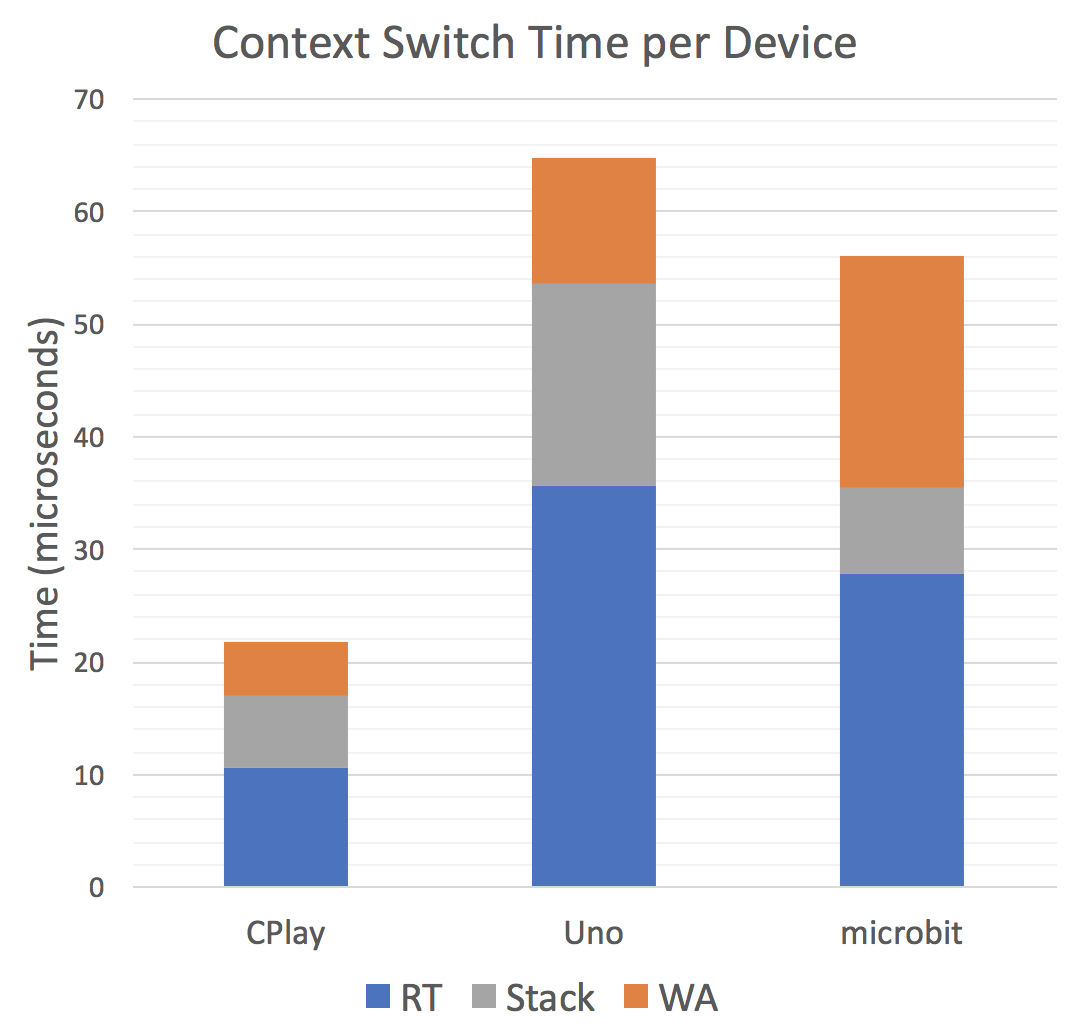
\includegraphics[width=.7\columnwidth]{images/context-switch.png}
\caption{\label{fig:context-switch}Base context switch profiles per device.}
\end{figure}

\begin{figure}[ht]
    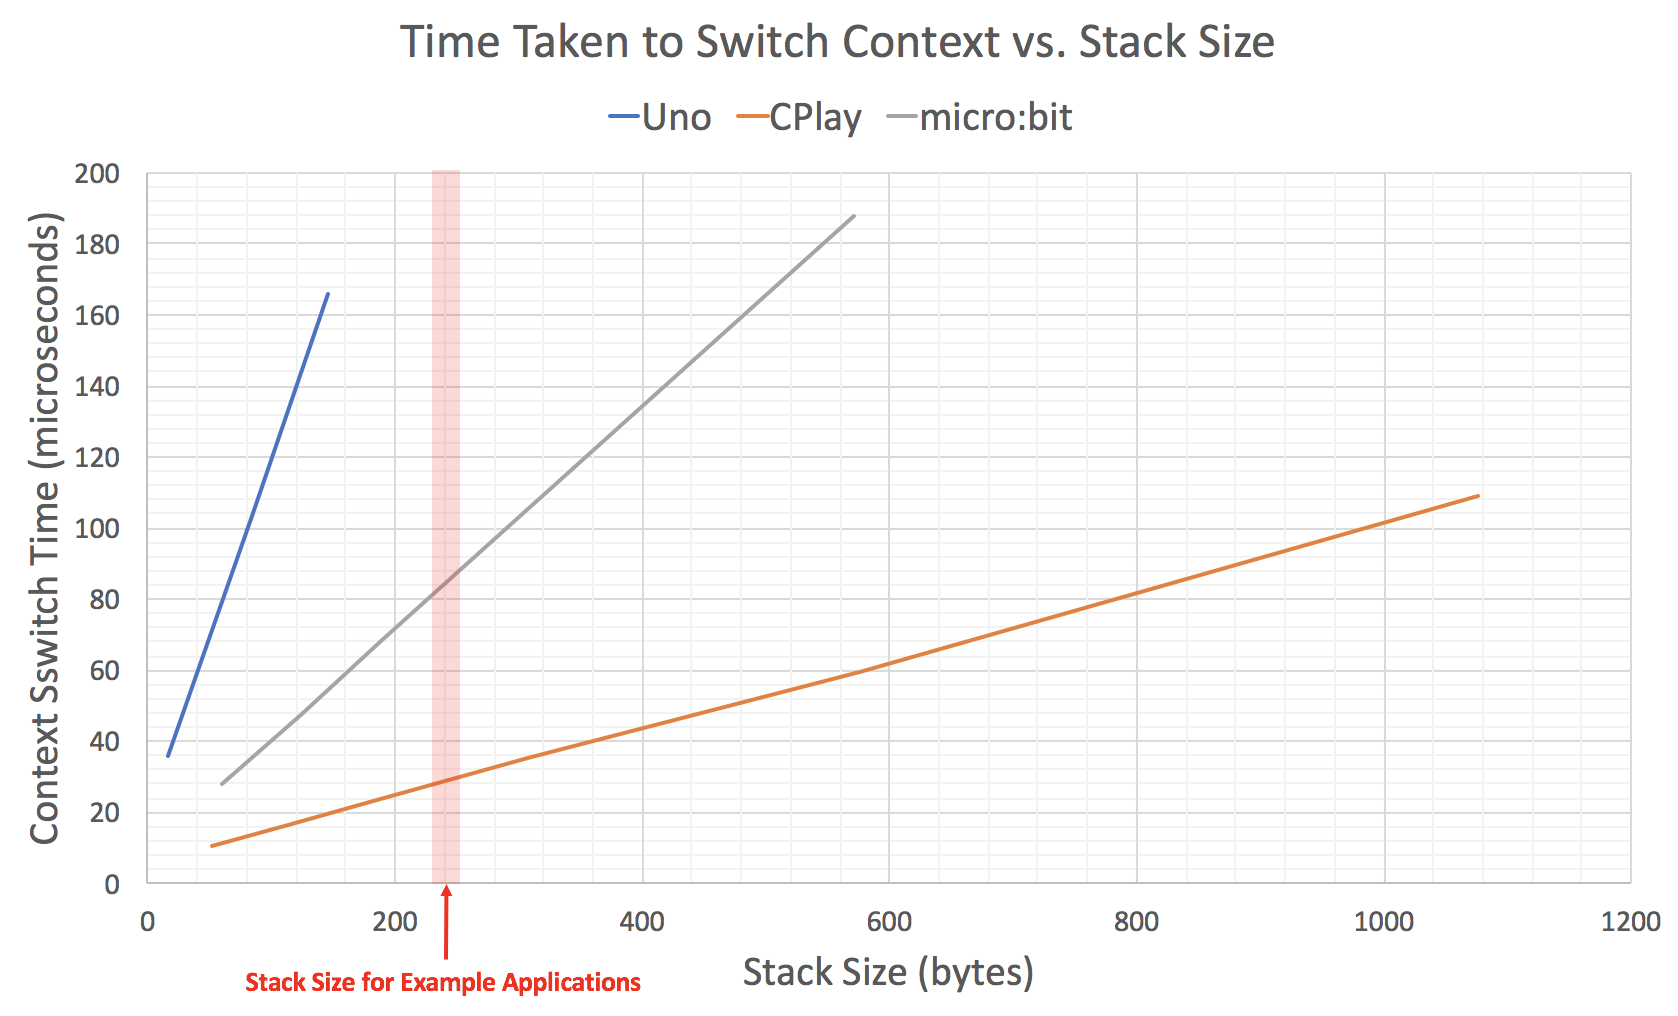
\includegraphics[width=.99\columnwidth]{images/context-vs-stack.png}
\caption{\label{fig:context-vs-stack}Time taken to perform a context switch against stack size.}
\end{figure}

To evaluate the performance of \CON's scheduler we conducted a test that created two fibers and continuously swapped context,
and the time taken to complete the context switch was measured. 
We performed this test in both STS and C++ and the resulting profiles can be seen in Figure~\ref{fig:context-switch}. 
This figure breaks the context switch down into three phases: 
(1) \CO, the time it takes to perform a context switch in \CO; 
(2) Stack, the time taken to page out the \MC stack; and 
(3) \MC, the overhead added by the \MC wrappers. 

From these results we can observe that context switches generally take of order tens of microseconds. 
The cost of \CON's stack paging approach can also be seen as a significant, but not dominant cost. 
The cost of stack paging would of course grow with stack depth.
Figure~\ref{fig:context-vs-stack} therefore profiles the time a context switch takes with an increasing stack size across all three devices in \CO. 
This test is similar to the previous test, however, we placed bytes (in powers of 2) on the stack of each fiber, starting from 64 and finishing at 1024. 
The difference in gradients, and ranges of values can be put down to device capability. 
For instance, the Uno has an 8-bit processor word size, which means more instructions are required to copy the stack, therefore as the stack size increases, so does context switch time. 
The vertical bands indicate typical stack sizes for \MC programs based on a representative set of examples.

%For the uno, the context switch profile is for the native implementation only.

\subsection{Performance of Asynchronous Operations}

\begin{table}[]
\centering
\begin{tabular}{c|c|c|}
    \cline{2-3}
                                                                                                                & \begin{tabular}[c]{@{}c@{}}RAM Overhead\\ (bytes)\end{tabular} & \begin{tabular}[c]{@{}c@{}}Processing Overhead\\ (microseconds)\end{tabular} \\ \hline
    \multicolumn{1}{|c|}{Create a Fiber}                                                                        & 136                                                            & 35.4                                                                         \\ \hline
    \multicolumn{1}{|c|}{\begin{tabular}[c]{@{}c@{}}Asynchronous \\ Procedure\\ Call\end{tabular}}              & 32                                                             & 4.01                                                                         \\ \hline
    \multicolumn{1}{|c|}{\begin{tabular}[c]{@{}c@{}}Asynchronous \\ Procedure\\ Call with a Sleep\end{tabular}} & 204                                                            & 32.4                                                                         \\ \hline
    \end{tabular}
\caption{\label{table:time-ram-consumption}RAM consumption and processing time for various asynchronous operations in \CO.}
\end{table}

To gauge the cost of asynchronous operations in \CON, we tested three commonly used code paths, designed to determine the efficiency of \CON's \emph{fork-on-block} Asynchronous Procedure Call (APC) mechanism that underpins all event handlers in \MC and \CO. We measure to RAM and processor cost of: (1) creating a fiber; (2) handling a non-blocking APC call; and (3) handling a blocking APC call. Table~\ref{table:time-ram-consumption} presents our results. Again, the Adafruit CPX device was used for this experiment.

These result highlight the performance gains of the opportunistic fork-on-block mechanism over a naiive approach that would would execute every event handlers in a separate fiber. For non-blocking calls, the best case, this has an small overhead of 32 bytes of RAM and is not processor intensive, versus the worst case, which incurs a large overhead of 204 bytes of RAM and 32.4 microseconds of processor time.

\subsection{Flash Memory Usage}

\begin{table}[]
\centering
\begin{tabular}{c|c|c|c|}
\cline{2-4}
                                                                                                & CPX & micro:bit & Uno  \\ \hline
\multicolumn{1}{|c|}{WA}                                                                       & 20.46 & 12.14     & 7.79 \\ \hline
\multicolumn{1}{|c|}{RT}                                                                       & 29.85 & 34.35     & 13.7 \\ \hline
\multicolumn{1}{|c|}{\begin{tabular}[c]{@{}c@{}}mbed and \\ Supporting Libraries\end{tabular}} & 14.99 & 24.28     & -    \\ \hline
\multicolumn{1}{|c|}{C++ Standard Library}                                                     & 43.14 & 24        & 1.03 \\ \hline
\end{tabular}

\caption{\label{table:flash-consumption}The total flash consumption of code required to support \MC (KB).}
\end{table}

MCU's make use of internal non-volatile FLASH memory to store program code. Table~\ref{table:flash-consumption} shows the per device flash consumption of each software library used in the final \MC binary. To obtain these numbers, we profiled the final map file produced after compilation. The ordering of the table aligns with the composition of the software layer: \MC builds on \CO which builds on the C++ standard library and optionally, mbed.

From the bottom up, the profile of the standard library changes dramatically for each device: The Uno has a very lightweight standard library; the microbit uses 64-bit integer operations (for timers) which requires extra standard library functions; and the CPX requires software floating point operations pulling in more standard library functions.

The size of \CO and \MC scales linearly with the amount of functionality a device has, due to the component oriented nature of \CO and transitively \MC. For instance the Uno has few onboard components when compared to the CPX and micro:bit. The modular composition of \CO allows us to support multiple devices with a variety of feature sets, whilst maintaining the same API at the \MC layer.

\subsection{RAM Memory Usage}

\begin{table}[]
\centering
\begin{tabular}{c|c|c|c|}
\cline{2-4}
                                                                                                & CPX & micro:bit & Uno   \\ \hline
\multicolumn{1}{|c|}{WA}                                                                       & 0.612 & 1.069     & 0.074 \\ \hline
\multicolumn{1}{|c|}{RT}                                                                       & 0.369 & 0.214     & 0.156 \\ \hline
\multicolumn{1}{|c|}{\begin{tabular}[c]{@{}c@{}}mbed and Supporting \\ Libraries\end{tabular}} & 0.312 & 0.923     & -     \\ \hline
\multicolumn{1}{|c|}{C++ Standard Library}                                                     & 0.161 & 0.149     & 0.074 \\ \hline
\end{tabular}
\caption{\label{table:ram-consumption}The total static ram consumption for an \MC binary (KB).}
\end{table}

Table~\ref{table:ram-consumption} shows the per device ram consumption of each software library used in the final \MC binary. To obtain these numbers, we profiled the final map file produced after compilation. At runtime MakeCode also dynamically allocates additional memory: 1.56 kB for the CPX, 560 bytes for the micro:bit, and 644 bytes for the Uno. From the table, we can see that in all cases, the RAM consumption of \MC+\CO is well within the RAM available of each device.

% Add globals maps and profile of listener and fiber.

% The CPX runtime is the largest, as the CPX device has lots of on-board
% components, and this runtime shares much of its code with other SAMD21 \MC targets.
% The compiled C++ runtime is 114k in total, with \CO accounting for 29k, with an
% additional 15k from libmbed. The \MCN-common-packages adds 20k, and also in
% an additional 49k of math support libraries (floating point operations,
% including trigonometry and number printing/parsing).
% As the SAMD21 has 256k of flash, we did not worry about optimizing this runtime for space.

% On the Uno, which has 32k of flash, the much \MC runtime is 8k and \CO is 14k (since
% the Uno only requires basic GPIO, i2c and serial drivers), leaving 10k for user code.

% The TypeScript part of the runtime is 1060 statements on the CPX and 216 on the Uno.
% In our microbenchmarks, 99\% of that runtime is tree-shaken away.

\subsection{Compiling Static TypeScript}

When compiling, the entire TypeScript program, including the runtime, is
passed to the TypeScript (TS) language service for parsing. Then, only the remaining part of the program (after code shaking) is compiled to native code.
On a modern laptop, using Node.js, TS parsing and analysis takes about 0.1ms per statement, and \MC compilation to native code takes about 1ms per statement.
While the TS compiler has been optimized for speed, \MCN's native compilation process hasn't been. For example, the CPX TS pass is dominated by compilation of the device runtime and takes about 100ms, whereas the \MC pass typically only includes a small user program and a small bit of the runtime, resulting in less than 100ms. Thus, typical compilation times are under 200ms for typical user programs of 100 lines or less.

% Not really a result, more of a description of design, with an anecdotal comment about speed.

% should be moved further up and described alongside AVR VM vs. Native

% The AVR VM was specifically designed for high code density, since \CO
% leaves less than 10k for TS runtime and user code on the Uno. The interpreter is implemented in assembly, always included with the program, and is around 0.5k.
% There are about 30 opcodes, some of which can take 1 or 2 byte arguments. There are also a few combined opcodes, representing a sequence of one argument-less opcode, and one with an argument, which improves code density by about 25\%. Opcodes are direct offsets into the code of the interpreter, speeding up execution. They operate on a stack (mainly for function calls) and a special scratch register. There is essentially no stack space overhead compared to native AVR compilation. The speed overhead is around 4x-5x (with respect to native) for computational tasks.


%\subsection{Implementation}
% •	\CO (SAMD21 and AVR): base runtime (C++ only)
% •	pxt
% •	pxt-common-packages: C++ and Static TypeScript
% •	pxt-adafruit
% •	pxt-arduino-uno
% •	pxt-monaco, pxt-blockly

%mmoskal [10:10 AM]
%`pxt checkdocs --snippets --re perf --stats`
% [10:11]
% I compile empty sample first twice, to reduce JIT costs
% [10:12]
% also, the first "compile prep" is slightly more costly, since it parses a hex file

    \section{Related Work}
\label{sec:related}

Related work breaks into four parts: the programming of microcontrollers, 
type systems for JavaScript, operating systems
for microcontrollers, and techniques for code loading.

\subsection{Programming microcontrollers}

\begin{itemize}
\item binary compiled on host computer and loaded; this is the common paradigm for Arduino;
\item command and control via host computer (Firmata, Bluetooth)
\item complete VM on microcontroller (MicroPython)
\end{itemize}

Web-based programming

\begin{itemize}
\item Arduino IDE
\item scratch and scratch extensions (provide tethered mode for microcontrollers)
\item 
\end{itemize}

\subsection{Types for JavaScript}

Type systems with soundness guarantees for JavaScript are numerous. 
Safe TypeScript~\cite{SafeTypeScript15}: distinguishes dynamic from Any type - dynamic means
one of the known static types, where as Any denotes types coming
from raw JavaScript.

StrongScript XYZ.
Static TypeScript differs from these efforts by XYZ. 

% Other ways to restrict JavaScript/TypeScript
% •	Safe TypeScript
% •	StrongScript
% •	Quite a few others…
% MicroPython

\subsection{Operating systems}

% https://state-machine.com/arduino/ 
% http://tinyos.stanford.edu/tinyos-wiki/index.php/TinyOS_Overview 

% Tethered modes: Kodu for micro:bit, Scratch for micro:bit. The PC is central, the microcontroller is peripheral
% Virtual machines: MicroPython, ev3, littlebits, etc.
% Raspberry Pi: complete operating system

\subsection{Code loading}

% ARM solution
    \section{Conclusion}
\label{sec:conclude}

Hardware partners already have started to create MakeCode packages for the micro:bit.
Seeed Studio (\url{https://www.seeedstudio.com/}) has created packages to add its Grove components to a micro:bit.
Grove components are accessed via the I2C serial protocol, supported by the micro:bit device runtime.
All micro:bit packages for the Grove components are authored in Static TypeScript (gesture, ultrasonic-ranger,
4-digital-display, two-led-matrix). These packages can be found under GitHub user ``Tinkertanker'', prefixed with
``pxt-''. Sparkfun has created MakeCode packages for its micro:bit shields (GitHub user ``sparkfun'').

% https://github.com/Tinkertanker/pxt-ssd1306-microbit
% https://github.com/Tinkertanker/pxt-ir-microbit 
% https://github.com/Tinkertanker/pxt-ky040-microbit
% https://github.com/Tinkertanker/pxt-ds1307-microbit
% Sparkfun
% •	https://github.com/sparkfun/pxt-weather-bit
% •	https://github.com/sparkfun/pxt-moto-bit 
% •	https://github.com/sparkfun/pxt-gamer-bit 
% Common packages
% •	https://github.com/Microsoft/pxt-common-packages
% •	Structure:
% o	Libs/package/
% [talk about C++] Various examples.
% [more about customer editor associated with a package]

    
    %% Bibliography
    \bibliography{paper}
    
    
    %% Appendix
    \appendix
    \section{Appendix}
    
    Text of appendix \ldots
    
    \end{document}
